% !TeX program = xelatex
% !TeX encoding = UTF-8
\documentclass[12pt,a4paper]{article}
\usepackage{fontspec}
\usepackage[top=2.54cm,bottom=5.7cm,left=3.18cm,right=3.18cm,headheight=0pt,headsep=0pt,footskip=4.66cm]{geometry}
\setmainfont{NotoSerifSC-Regular.ttf}[Path=build-fonts/,BoldFont=NotoSerifSC-Bold.ttf]
\newfontfamily\headingfont{NotoSansSC-Regular.ttf}[Path=build-fonts/]
\newcommand{\songti}{\normalfont}
\newcommand{\heiti}{\headingfont}
\XeTeXlinebreaklocale "zh"
\XeTeXlinebreakskip=0pt plus 1pt
\usepackage{amsmath,amssymb,mathtools,bm}
\renewcommand{\theequation}{\arabic{equation}}
\usepackage{graphicx}
\usepackage{longtable,booktabs,array,tabularx,calc}
\usepackage{etoolbox}
\usepackage{float}
\usepackage{needspace}
\usepackage{caption}
\usepackage{setspace}
\usepackage{fancyhdr}
\usepackage{titlesec}
\usepackage{tocloft}
\usepackage{indentfirst}
\usepackage{enumitem}
\usepackage{fvextra}
\usepackage{xcolor}
\usepackage{xurl}
\usepackage[hidelinks]{hyperref}
\usepackage{bookmark}
\usepackage{eso-pic}
\usepackage{tikz}
\usetikzlibrary{positioning,arrows.meta,shapes.geometric,fit,backgrounds,calc}
\newcommand{\R}{\mathbb{R}}
\newcommand{\Bset}{\{0,1\}}
\DeclareMathOperator*{\argmin}{arg\,min}
\definecolor{paperGreen}{RGB}{132,168,60}
\definecolor{paperGreenDark}{RGB}{79,96,48}
\definecolor{paperGreenLight}{RGB}{212,224,192}
\definecolor{paperCream}{RGB}{245,243,232}
\tikzset{
  startstop/.style={rectangle,rounded corners=8pt,minimum width=3.2cm,minimum height=0.9cm,align=center,draw=paperGreenDark,fill=paperGreen,text=white,thick},
  process/.style={rectangle,minimum width=3.6cm,minimum height=0.9cm,align=center,draw=paperGreenDark,fill=paperCream,thick},
  decision/.style={diamond,aspect=2.1,minimum width=3.0cm,align=center,draw=paperGreenDark,fill=paperGreenLight,thick,inner sep=1pt},
  data/.style={trapezium,trapezium left angle=70,trapezium right angle=110,minimum width=3.2cm,minimum height=0.9cm,align=center,draw=paperGreenDark,fill=paperGreenLight!55,thick},
  verify/.style={rectangle,minimum width=3.4cm,minimum height=0.9cm,align=center,draw=paperGreenDark,fill=paperGreenLight,thick},
  layer/.style={rectangle,draw=paperGreenDark,dashed,inner sep=6pt},
  arrow/.style={-{Stealth[length=2.4mm]},thick,draw=paperGreenDark},
  lab/.style={font=\small,midway}
}
\newcommand{\sanhao}{\fontsize{16pt}{16pt}\selectfont}
\newcommand{\xiaosan}{\fontsize{15pt}{18.75pt}\selectfont}
\newcommand{\sihao}{\fontsize{14pt}{14pt}\selectfont}
\newcommand{\xiaosi}{\fontsize{12pt}{12pt}\selectfont}
\newcommand{\wuhao}{\fontsize{10.5pt}{10.5pt}\selectfont}
% 正文参考文献编号采用右上角标注
\newcommand{\supcite}[1]{\textsuperscript{[#1]}}

\AtBeginDocument{%
  \xiaosi\songti\setstretch{1.25}%
  % 统一所有行间公式与上下正文之间的距离
  \setlength{\abovedisplayskip}{7.5pt}%
  \setlength{\belowdisplayskip}{7.5pt}%
  \setlength{\abovedisplayshortskip}{7.5pt}%
  \setlength{\belowdisplayshortskip}{7.5pt}%
}
\setstretch{1.25}
\setlength{\parindent}{2em}
\setlength{\parskip}{7.5pt}
\pagestyle{fancy}
\fancyhf{}
\fancyfoot[C]{\xiaosi\thepage}
\renewcommand{\headrulewidth}{0pt}
\renewcommand{\footrulewidth}{0pt}
\fancypagestyle{plain}{\fancyhf{}\fancyfoot[C]{\xiaosi\thepage}\renewcommand{\headrulewidth}{0pt}\renewcommand{\footrulewidth}{0pt}}
\newcommand{\ChineseNumber}[1]{%
  \ifcase#1 零\or 一\or 二\or 三\or 四\or 五\or 六\or 七\or 八\or 九\or 十%
  \or 十一\or 十二\or 十三\or 十四\or 十五\or 十六\or 十七\or 十八\or 十九\or 二十\else #1\fi}
\renewcommand{\thesection}{\ChineseNumber{\value{section}}、}
\renewcommand{\thesubsection}{（\ChineseNumber{\value{subsection}}）}
\renewcommand{\thesubsubsection}{（\arabic{subsubsection}）}
\renewcommand{\theparagraph}{（\arabic{paragraph}）}
\renewcommand{\thesubparagraph}{\arabic{subparagraph}）}
\titleformat{\section}{\centering\heiti\xiaosan}{\thesection}{0.5em}{}
\titlespacing*{\section}{0pt}{12pt}{6pt}
\titleformat{\subsection}{\raggedright\heiti\sihao}{\thesubsection}{0.5em}{}
\titlespacing*{\subsection}{0pt}{6pt}{0pt}
\titleformat{\subsubsection}{\raggedright\songti\xiaosi\bfseries}{\thesubsubsection}{0.5em}{}
\titlespacing*{\subsubsection}{0pt}{6pt}{0pt}
\titleformat{\paragraph}[runin]{\raggedright\songti\xiaosi}{\theparagraph}{0.5em}{}
\titleformat{\subparagraph}[runin]{\raggedright\songti\xiaosi}{\thesubparagraph}{0.5em}{}
\setcounter{secnumdepth}{5}
\setcounter{tocdepth}{3}
% 目录按标题层级逐级缩进：一级顶格，二级和三级依次右移
\cftsetindents{section}{0em}{4em}
\cftsetindents{subsection}{0em}{4em}
\cftsetindents{subsubsection}{0em}{4em}
\makeatletter
\let\paper@l@subsection\l@subsection
\let\paper@l@subsubsection\l@subsubsection
\renewcommand*{\l@subsection}[2]{\paper@l@subsection{\hspace*{2em}#1}{#2}}
\renewcommand*{\l@subsubsection}[2]{\paper@l@subsubsection{\hspace*{4em}#1}{#2}}
\makeatother
\renewcommand{\figurename}{图}
\renewcommand{\tablename}{表}
\DeclareCaptionFont{captioncn}{\songti\xiaosi\setstretch{1.0}}
\DeclareCaptionLabelSeparator{twospaces}{\hspace{2em}}
\captionsetup{font=captioncn,labelsep=twospaces,justification=centering,singlelinecheck=true}
\captionsetup[table]{position=top}
\captionsetup[figure]{position=bottom}
\renewcommand{\thefootnote}{\textcircled{\scriptsize\arabic{footnote}}}
\graphicspath{{media/}}
\makeatletter
\def\maxwidth{\ifdim\Gin@nat@width>\linewidth\linewidth\else\Gin@nat@width\fi}
\def\maxheight{\ifdim\Gin@nat@height>0.82\textheight 0.82\textheight\else\Gin@nat@height\fi}
\def\fps@figure{htbp}
\setlength{\@fptop}{0pt}
\setlength{\@fpsep}{12pt plus 2pt}
\setlength{\@fpbot}{0pt plus 1fil}
\patchcmd\longtable{\par}{\if@noskipsec\mbox{}\fi\par}{}{}
\makeatother
\AtBeginEnvironment{tabular}{\songti\xiaosi\setstretch{1.0}}
\AtBeginEnvironment{longtable}{\songti\xiaosi\setstretch{1.0}}
\setkeys{Gin}{width=\maxwidth,height=\maxheight,keepaspectratio}
\setlength{\emergencystretch}{3em}
\renewcommand{\arraystretch}{1.15}
\renewcommand{\topfraction}{0.9}
\renewcommand{\textfraction}{0.08}
\renewcommand{\floatpagefraction}{0.75}
\providecommand{\tightlist}{\setlength{\itemsep}{0pt}\setlength{\parskip}{0pt}}
\urlstyle{same}
\hypersetup{pdfauthor={},pdftitle={暖城向新·热力不息}}

\newcommand{\EnableBodyBackground}{%
  \AddToShipoutPictureBG{%
    \AtPageLowerLeft{%
      
\includegraphics[width=\paperwidth,height=\paperheight]{body-background.jpg}%
    }%
  }%
}

\newenvironment{refsectionflush}
  {\par\sloppy\setlength{\parindent}{0pt}\setlength{\parskip}{0pt}}
  {\par\fussy}
\newcommand{\refentry}[2]{%
  \par\noindent\hangindent=2em\hangafter=1
  [#1]\enspace #2\par}

\pretocmd{\section}{\clearpage}{}{}
\widowpenalty=10000\clubpenalty=10000
\begin{document}

\AddToShipoutPictureBG*{%
  \AtPageLowerLeft{
\includegraphics[width=\paperwidth,height=\paperheight]{cover.jpg}}%
}
\thispagestyle{empty}
\null
\clearpage
\EnableBodyBackground
\pagestyle{empty}
\begin{center}
{\songti\sanhao\bfseries\setstretch{1.0} 暖城向新·热力不息\par}
\vspace{6pt}
{\songti\xiaosi 面向多气候场景的供热源荷协同规划与物理约束优化\par}
\vspace{12pt}
{\heiti\sihao 摘\quad 要\par}
\end{center}
\vspace{3pt}
\par\indent 供热规划既要满足建筑的用热需求，也要考虑热源、管网和配电容量的限制。本文以乌鲁木齐、固原和武汉为背景，将热源、管网、建筑负荷与储热设备纳入同一模型。模型分别计算余热取用、设备供热和耗电，并用室温变化描述提前供热的作用。求解时，在保持总能量的条件下调整代表日权重；通过改变碳排放上限比较费用；对不满足管网温度和压力要求的运行方式，自动排除后重新计算。

在六栋建筑的外部实测负荷上，代表日的归一分布误差中位数由12.32\%降至4.48\%，通过全部统计检查的案例由3个增至4个。采用厂家165对制热量与输入功率数据，三城六组实验在相同设备和舒适要求下运行2880小时，优化方案较逐时温控策略降低电量费约1.10\%--1.60\%。双建筑对照中，将一栋建筑热容增至四倍后，节费比例由无区域用电上限时的7.22\%降至有上限时的4.66\%。四楼历史数学场景完成8784小时服务年回放；72小时参考管网经三轮反馈满足温压要求。

三城费用与碳排放的折中方案将最低电费方案相对基准的额外排放约减半，同时保留其80.92\%--89.44\%的节费金额。结果说明，提前供热可以利用低价电，但其价值取决于设备能力、热损和区域容量。本文在公开数据与公共原型条件下，给出了可复算的方案比较方法。

\vspace{-4.5pt}
\noindent{\heiti\xiaosi 关键词：}{\songti\xiaosi 源网荷储；建筑热惯性；多目标规划；代表日校正；物理反馈}
\clearpage
\thispagestyle{empty}
\begin{center}{\heiti\sihao 目\quad 录}\end{center}
\begingroup
\fontsize{10.5pt}{12pt}\selectfont\setstretch{1.0}
\setlength{\parskip}{0pt}
\setlength{\cftbeforesecskip}{1pt}
\makeatletter
\@starttoc{toc}
\makeatother
\endgroup
\clearpage
\pagenumbering{arabic}
\setcounter{page}{1}
\pagestyle{fancy}
% !TeX root = ../main.tex
% !TeX program = xelatex
% !TeX encoding = UTF-8
\section{研究问题与技术贡献}

供热规划需要确定设备配置、逐时运行及费用与排放的取舍。余热要满足温度和输送条件，热泵要在低温时保持出力，多楼预热还会竞争区域用电容量，三者需要联合计算。

建筑热动态模型能够描述供热对后续室温的影响\supcite{2}；典型时段方法缩减计算规模，但需处理蓄热状态的时序联系\supcite{4}；$\varepsilon$约束方法通过改变目标上限比较方案\supcite{5}。本文重点研究这些方法在供热问题中的衔接：压缩后保留什么负荷特征，预热占用多少容量，以及方案能否满足设备和管网要求。

按赛事要求\supcite{1}，以乌鲁木齐、固原和武汉为背景，将热源、管网、建筑负荷与储热设备纳入源—网—荷—储模型，形成四项工作。

第一，统一热量计量。直接换热与热泵共用的余热只计一次，热泵源侧取热和电功分开计算；逐楼室温、储热量与系统电力共同约束运行。

第二，校正代表日权重。代表日是选出的实际日期，权重表示折合天数。在日数和能量守恒下调整权重，使负荷分布接近原序列，同时检查峰值和相邻小时的最大变化。

第三，将工程条件反馈给优化。厂家同工况制热量和输入功率同时限制出力与耗电；不满足远端温度或压降要求的管网模式被排除后重算，保存调整原因与费用。

第四，通过对照解释决策收益。完整服务年回放检验连续运行；同设备策略、热容与配电上限、碳帽和采购预算对照分别识别节费机制及方案切换条件。

\section{数据基础与三城实验设计}
\subsection{数据来源和用途}

模型输入包括天气、建筑参数、负荷记录、设备性能和费用因子。每份资料保留来源、所属对象与时间范围，计算得到的参数同时保留换算过程。表\ref{tab:data-scope}列出它们在实验中的用途，区分实测负荷、公共建筑原型和模型计算值。

\begin{table}[htbp]
\centering
\caption{研究数据及其用途}\label{tab:data-scope}
\begin{tabularx}{\textwidth}{@{}>{\raggedright\arraybackslash}p{0.23\textwidth}X >{\raggedright\arraybackslash}p{0.23\textwidth}@{}}
\toprule
数据来源 & 在本文中的作用 & 数据类型\\
\midrule
NASA POWER逐时气象\supcite{9} & 三城同一时间段的天气输入；统一时区与单位 & 公开气象网格数据\\
BESTEST 600原型\supcite{11} & 建筑几何与热工参数的来源；用于推导简化热模型参数 & 公共原型的派生参数\\
BDG2建筑计量\supcite{10} & 六栋建筑的负荷压缩与代表日权重对照 & 外部计量基准\\
TICA产品样本\supcite{12} & 两型号共165个制热量/功率点及缺测角点 & 厂家公开工况表\\
电价及排放因子\supcite{13,14} & 在共同计费条件下比较电量费与碳排放 & 公开价格和核算因子\\
OSM空间数据 & 三城建筑与道路候选的空间参考 & 公开空间数据\\
\bottomrule
\end{tabularx}
\end{table}

三城气候对照从北京时间2024年11月16日00:00开始，到2025年3月16日00:00结束，不含终点时刻，共120日、2880个连续小时。各城采用相同建筑和室温要求，仅更换天气输入。费用统一按湖北工商业分时电价计算，碳排放统一由用电量乘固定平均排放因子得到，以便比较天气和调度的影响。这里得到的是共同计费条件下的结果。厂家热泵实验由48~m$^2$公共原型按20倍规模构造960~m$^2$计算对象，允许室温在20--27~$^\circ$C内变化，开始与结束时均为20~$^\circ$C。

三城公共原型用于气候与调度对照，六栋外部计量建筑用于检验负荷压缩，分别报告结果。

\subsection{三类场景与验证分工}

乌鲁木齐关注工业余热和集中输配，固原关注低温设备与清洁替代，武汉关注冷热需求及多楼协同。三城参与同窗调度对照；网络反馈用72小时参考系统，热容交互用武汉双楼算例。另保留武汉四楼、两区域的历史数学场景：2023年7月1日至2024年7月1日的8784小时服务年，包含2023年11月15日至2024年3月16日的2928小时声明冬季。日期均为北京时间、含起点不含终点；该冬季是项目服务假定。

BDG2数据来自境外建筑，其实测负荷用于评价压缩误差。三城OSM数据提供建筑位置和候选道路路径；热源能力、供热对象与逐时出力则由模型配置确定，不能仅从道路或建筑轮廓推得。

表\ref{tab:experiment-design}列出各实验固定了什么、改变了什么，以及由此能够判断什么。

\begin{table}[htbp]
\centering
\caption{主要实验的控制变量与验证任务}\label{tab:experiment-design}
\begin{tabularx}{\textwidth}{@{}>{\raggedright\arraybackslash}p{0.19\textwidth}XX@{}}
\toprule
实验对象 & 保持一致的条件 & 改变因素及验证任务\\
\midrule
六栋计量建筑 & 观测序列、各楼实际日集合 & 权重方法；检验分布保真与统计准入\\
三城两型号设备 & 各组天气、整机配置与温度服务 & 调度策略；识别同资产运行收益\\
武汉四楼两区域 & 合成参数、既定资产及舒适要求 & 完整服务年及声明冬季回放；检验连续状态\\
武汉双建筑 & 传热系数、天气与设备 & 热容倍率及公用电上限；识别交互作用\\
72小时参考管网 & 交付需求与物理校核阈值 & 可用模式目录；量化反馈修正及费用\\
三城理想资产 & 各城天气、资产与服务条件 & 碳排上限；比较降费、碳排与峰值\\
条件投资案例 & 2880小时服务与性能假设 & 设备台数、采购预算；确定选择阈值\\
\bottomrule
\end{tabularx}
\end{table}

\subsection{统一比较与计量规则}

每组对照仅改变待研究的因素，其余条件按表\ref{tab:experiment-design}保持一致。功率、能量、费用与排放分别用kW、kWh、元与kg计量。代表日权重用于汇总费用和能量；检验室温或储热量能否连续变化时，仍按真实时间顺序计算。程序检查年份、时区及小时是否连续，并保存配置、文件校验码、求解状态和独立复算结果，以确定每个数值对应的输入与计算过程。

% !TeX root = ../main.tex
% !TeX program = xelatex
% !TeX encoding = UTF-8
\section{源—网—荷—储与建筑热状态的统一模型}

模型把资源可用量、设备与管网交付能力及建筑舒适要求共同约束，决定新增或退役容量和逐时运行量，并递推室温与储热量。功率采用kW，热量采用kWh，温度采用$^\circ$C，温差采用K；时间步长$\Delta t$采用h，连续案例取$1~\mathrm h$。

\begin{figure}[htbp]
\centering
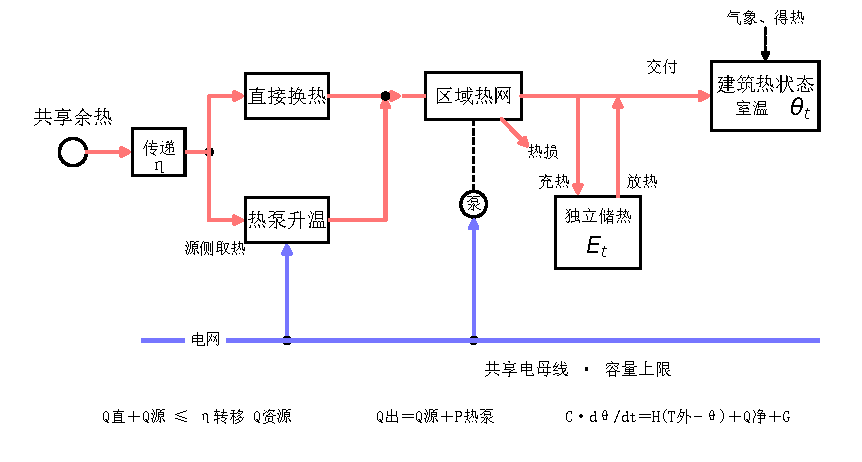
\includegraphics[width=\linewidth]{paper_r2/model_paper/source_network_load_storage_zh.pdf}
\caption{共享资源、热电网络与两类状态的统一结构。热泵源侧取热与电功分别计量；独立储热$E_t$与建筑室温$\theta_t$分别递推。各实验按配置启用模块。}
\label{fig:unified-structure}
\end{figure}

\subsection{资产容量与共享热资源}

温位表示用户所需的供水温度等级。同一设备向各温位的出力之和受可用容量限制。下文以$k,n,g,b,s,e,t$分别表示设备、区域节点、供热温位、建筑、储热装置、管段和时段。设备容量及出力满足
\begin{equation}
K_k=K_k^{\mathrm{exist}}+K_k^{\mathrm{new}}-K_k^{\mathrm{ret}},
\qquad
0\leq\sum_g Q_{k,g,t}\leq a_{k,t}K_k .
\label{eq:scoring-capacity}
\end{equation}
其中$K_k$为额定容量，三个上标分别表示现有、新增与退役容量；$Q_{k,g,t}$为向温位$g$供热的功率，$a_{k,t}$为逐时可用率。新增、退役、启停、最小出力及爬坡限制按设备配置设置。

直接换热与热泵共用余热时，须合计两类设备的取热量。热泵性能系数$\mathrm{COP}$为供热量与输入电量之比，其供热量扣除电功后才是源侧取热量。资源池$r$满足
\begin{equation}
R_{r,t}^{\mathrm{use}}
=\frac{1}{\eta_r^{\mathrm{tr}}}
\left[
\sum_{k\in\mathcal D_r,g}Q_{k,g,t}
+\sum_{k\in\mathcal H_r,g}
\left(1-\frac{1}{\mathrm{COP}_{k,g,t}}\right)Q_{k,g,t}
\right]
\leq \overline R_{r,t}.
\label{eq:scoring-resource}
\end{equation}
$R_{r,t}^{\mathrm{use}}$与$\overline R_{r,t}$分别为实际取用量和可用上限，$\eta_r^{\mathrm{tr}}\in(0,1]$为资源端至设备端的传热效率，$\mathcal D_r$与$\mathcal H_r$分别为直接换热和热泵设备集合。两类设备共用逐时资源限额，每个设备与资源池唯一关联，防止同一份余热被重复利用。资源传热、设备转换及管网输送的损失分别计算。

\subsection{设备性能域与温位适配}

通用模型按逐时工况给定$\mathrm{COP}$、制冷能效比$\mathrm{EER}$及转换效率；$\mathrm{EER}$为供冷量与输入电量之比。热泵与电锅炉分别满足
\begin{equation}
Q^{\mathrm{HP}}=\mathrm{COP}\,P^{\mathrm{HP}},\qquad
Q^{\mathrm{EB}}=\eta^{\mathrm{EB}}P^{\mathrm{EB}} .
\label{eq:scoring-conversion}
\end{equation}
其中$Q$为供热功率，$P$为输入电功率，上标$\mathrm{HP}$与$\mathrm{EB}$分别表示热泵和电锅炉，$\eta^{\mathrm{EB}}$为电锅炉效率。直接热源须满足用户供水温度要求；热泵升温后可接入更高温位。

设备性能域指厂家数据允许评价的工况范围。相应算例采用厂家表中同型号、同工况的供热功率$Q^{\mathrm{cat}}$与输入功率$P^{\mathrm{cat}}$，在相邻工况点间分别插值，再计算二者比值：
\begin{equation}
\begin{aligned}
Q_t^{\mathrm{cat}}&=\sum_i\lambda_{i,t}Q_i,\qquad
P_t^{\mathrm{cat}}=\sum_i\lambda_{i,t}P_i,\\
\mathrm{COP}_t^{\mathrm{cat}}&=\frac{Q_t^{\mathrm{cat}}}{P_t^{\mathrm{cat}}},\qquad
\lambda_{i,t}\geq0,\quad \sum_i\lambda_{i,t}=1 .
\end{aligned}
\label{eq:scoring-performance}
\end{equation}
其中$Q_i,P_i$为厂家表中工况点$i$的成对功率，$\lambda_{i,t}$由给定环境温度和出水温度确定。插值所需各点须有效且属于同型号，缺点、越界或跨型号组合不能参与优化。对工况有效的时段，固定整机算例以交付能力系数$\phi\in(0,1]$折减供热上限：
\begin{equation}
0\leq Q_t^{\mathrm{HP}}\leq\phi Q_t^{\mathrm{cat}},\qquad
P_t^{\mathrm{HP}}=
\frac{P_t^{\mathrm{cat}}}{\phi Q_t^{\mathrm{cat}}}Q_t^{\mathrm{HP}} .
\label{eq:scoring-duty}
\end{equation}
式\eqref{eq:scoring-duty}限定供热能力与单位耗电。理想小时占空比用小时内运行时间比例折算平均出力和耗电，不描述启停瞬态；型号、单位和工况随记录保存。

\subsection{节点守恒与网络物理反馈}

零失供时，节点按温位逐时平衡热源供热、管段输送、建筑用热和储热充放：
\begin{multline}
\sum_{k\in\mathcal K_n}Q_{k,g,t}
+\sum_{e\in\delta^-(n)}\eta_{e,t}F_{e,g,t}
+\sum_{s\in\mathcal S_{n,g}}Q_{s,t}^{\mathrm{dis}}\\
=D_{n,g,t}+\sum_{b\in\mathcal B_{n,g}}Q_{b,t}^{\mathrm h}
+\sum_{s\in\mathcal S_{n,g}}Q_{s,t}^{\mathrm{ch}}
+\sum_{e\in\delta^+(n)}F_{e,g,t}.
\label{eq:scoring-node}
\end{multline}
$\mathcal K_n$、$\mathcal S_{n,g}$和$\mathcal B_{n,g}$分别为相应设备、储热和建筑集合，$\delta^-(n)$与$\delta^+(n)$分别为流入和流出管段。$F$为管段入口功率，$\eta_{e,t}$为交付效率；$Q^{\mathrm{ch}}$与$Q^{\mathrm{dis}}$为充、放热功率，$Q_b^{\mathrm h}$为建筑实际受热功率。$D$只含建筑热状态模块未覆盖、且已计入需求侧调整的固定负荷，避免与建筑交付量重复计入。双向管段按实际方向计算，容量与改造状态限制输送，循环泵耗电计入系统电负荷。

热量够用还不代表远端供水温度和输送压力合格。对各支路独立设泵的星型管网，模型只采用有限个稳态模式；每个模式$m$给定流量和回水温度，并计算双管散热、水力阻力及泵功率：
\begin{equation}
\eta_m^{\mathrm{net}}=\frac{Q_m^{\mathrm{out}}}{Q_m^{\mathrm{in}}},
\qquad
P_m^{\mathrm{pump}}=
\frac{\Delta p_m\dot m_m}{1000\,\rho\,\eta_m^{\mathrm{pump}}}.
\label{eq:scoring-network}
\end{equation}
其中$Q_m^{\mathrm{in}}$与$Q_m^{\mathrm{out}}$为入口和出口热功率，其比值为输送效率；$\Delta p_m$为压差（Pa），$\dot m_m$为质量流量（kg/s），$\rho$为水密度（kg/m$^3$），$\eta_m^{\mathrm{pump}}$为泵效率，$P_m^{\mathrm{pump}}$为泵功率。求解后检查模式开启时的远端温度、流速、压降和泵功率，禁用不合格模式后重新求解。

\subsection{建筑热状态与精确逐时递推}

提前供热通过建筑蓄热影响后续室温，也增加散热。建筑采用1R1C结构\supcite{2}：等效热阻表示与室外的传热阻力，等效热容表示蓄热能力，室温是唯一状态。其变化满足
\begin{align}
C_b\frac{\mathrm d\theta_b}{\mathrm dt}
&=H_b(T^{\mathrm{out}}-\theta_b)+Q_b^{\mathrm h}-Q_b^{\mathrm c}+G_b,
\label{eq:scoring-rc-cont}\\
a_b&=\exp(-H_b\Delta t/C_b),\qquad
\beta_b=(1-a_b)/H_b,\\
\theta_{b,t}
&=a_b\theta_{b,t-1}+(1-a_b)T_t^{\mathrm{out}}
+\beta_b(Q_{b,t}^{\mathrm h}-Q_{b,t}^{\mathrm c}+G_{b,t}).
\label{eq:scoring-rc}
\end{align}
$\theta_b$为室温，$T^{\mathrm{out}}$为室外温度；$H_b$为围护与换气的总热损失系数（kW/K），$C_b$为等效热容（kWh/K）。$Q_b^{\mathrm h}$与$Q_b^{\mathrm c}$为供热和供冷功率，$G_b$为内部与太阳得热之和（kW）。$a_b$表示上一时段室温影响的保留程度，$\beta_b$表示净得热对室温的影响。式\eqref{eq:scoring-rc}是每时段输入保持不变时的精确积分，$\theta_{b,t}$为时段末室温。

室温受逐时舒适上下界约束，冷热受功率上限约束；启用互斥时，用二元变量排除同楼同时供热、供冷。建筑交付进入式\eqref{eq:scoring-node}，预热占用设备和配电容量，并增加散热。给定初温连续递推至规定终温或区间；方案比较固定舒适及初末态，避免透支末态蓄热，逐楼室温与交付量导出后复算。

给定目标室温时，可由式\eqref{eq:scoring-rc}反解所需净供热功率；本文在舒适带内联合选择室温与供热功率，使负荷随调度而变化。

\subsection{独立储热的连续性与边界}

独立储热以存量$E_{s,t}$表示，每时段扣损后加充热、减放热。以下$t=1,\ldots,T$，$E_{s,0}$为首小时开始前的存量，$K_s^E$为现有与新增能量容量，$r_s$为功率能量比（h$^{-1}$），则
\begin{align}
E_{s,t}
&=(1-\mu_s)^{\Delta t}E_{s,t-1}
+\eta_s^{\mathrm{ch}}Q_{s,t}^{\mathrm{ch}}\Delta t
-Q_{s,t}^{\mathrm{dis}}\Delta t/\eta_s^{\mathrm{dis}},
\label{eq:scoring-storage}\\
0\leq E_{s,t}&\leq K_s^E,\qquad
0\leq Q_{s,t}^{\mathrm{ch}},Q_{s,t}^{\mathrm{dis}}\leq r_sK_s^E .
\end{align}
$\mu_s$为每小时自损失率，$\eta_s^{\mathrm{ch}}$与$\eta_s^{\mathrm{dis}}$为充、放热效率；严格模式用二元变量约束充放互斥。$f_s^{\mathrm{init}}$与$f_s^{\mathrm{final}}$为初始和末端容量比例。固定初态采用$E_{s,0}=f_s^{\mathrm{init}}K_s^E$，组末要求$E_{s,\mathrm{end}}\geq f_s^{\mathrm{final}}K_s^E$；循环边界连接组首与组末。状态逐时递推，代表期权重只累计费用和能量，不放大状态变化。厂家与双楼机制实验不设独立储热，以识别建筑自身的调节作用。

\subsection{共享电力与多尺度耦合}

电驱热源、制冷设备和循环泵共用配电容量，其功率合计为系统电负荷：
\begin{align}
P_t^{\mathrm{sys}}
&=\sum_{k,g}\frac{Q_{k,g,t}^{\mathrm{HP}}}{\mathrm{COP}_{k,g,t}}
+\sum_k\frac{Q_{k,t}^{\mathrm{EB}}}{\eta_k^{\mathrm{EB}}}
\notag\\
&\quad+\sum_k\frac{Q_{k,t}^{\mathrm c}}{\mathrm{EER}_{k,t}}
+\sum_eP_{e,t}^{\mathrm{pump}},
\notag\\
(1+\sigma)P_t^{\mathrm{sys}}&\leq a_t^{\mathrm{grid}}K^{\mathrm{grid}}.
\label{eq:scoring-electric}
\end{align}
$P_t^{\mathrm{sys}}$为系统总电功率，$\sigma$为备用裕度，$K^{\mathrm{grid}}$为接入容量，$a_t^{\mathrm{grid}}$为逐时可用率。该式用于无微电网情形；启用微电网时，充电增加进口需求，本地发电与放电减少进口需求，进口须非负。系统接入容量限制区域合计电功率，区域节点向各楼交付热量，各楼室温约束所需冷热量。共享上限绑定时，一楼预热会减少其他楼的可用电功。

\subsection{费用与系统碳排放的统一核算}

费用和碳排放使用同一份调度量及时间权重。设$\omega_t=\pi_t w_t\Delta t$，其中$\pi_t$为情景概率，$w_t$为代表期对应的出现次数权重，核算式为
\begin{equation}
\begin{aligned}
C_0={}&\mathrm{CRF}\,I_{\mathrm{net}}+C_{\mathrm{fix}}+C_{\mathrm{event}}+C_{\mathrm{basic}}+C_{\mathrm{other}}
+\sum_t\omega_t\,\boldsymbol c_t^\mathsf T\boldsymbol x_t,\\
\mathcal E={}&\mathcal E_{\mathrm{const}}+\sum_t\omega_t\,\boldsymbol e_t^\mathsf T\boldsymbol x_t .
\end{aligned}
\label{eq:scoring-ledger}
\end{equation}
$C_0$为基本费用（元），$\mathcal E$为系统碳排放（kg），$\boldsymbol x_t$为逐时运行变量向量；$\boldsymbol c_t$与$\boldsymbol e_t$为相应费用和排放系数。$\mathrm{CRF}$为投资年化系数，将扣除补贴后的净投资$I_{\mathrm{net}}$折算为年费用；$C_{\mathrm{fix}}$为固定费用，其余费用项分别对应启停、基本电费及其他启用费用，$\mathcal E_{\mathrm{const}}$为排放常数项。后文采用$F_C=C_0+C_{\mathrm{carbon}}+C_{\mathrm{pref}}$、$F_E=\mathcal E$，其中新增项为碳费用与偏好惩罚。供热、供冷和共享电力的排放合计后受碳帽约束，即不得超过给定排放额度。

地源设备按地源$j$和情景累计供热取热量$E_j^{\mathrm{ext}}$与供冷排热量$E_j^{\mathrm{rej}}$，分别扣除与计入压缩机电耗。启用年度比例时，以$r_j^{\min}$与$r_j^{\max}$限制两者比例：
\begin{equation}
r_j^{\min}E_j^{\mathrm{rej}}\leq E_j^{\mathrm{ext}}
\leq r_j^{\max}E_j^{\mathrm{rej}} .
\label{eq:ground-ledger}
\end{equation}

% !TeX root = ../main.tex
% !TeX program = xelatex
% !TeX encoding = UTF-8
\section{多目标规划与物理反馈求解}

\subsection{费用与系统碳的容差端点及约束扫描}

技术、管网和运行模式是离散选择，能流、容量与热状态为连续变量，共同构成混合整数线性规划（MILP）。费用和系统碳排放由同一份运行量计算，目标为
\begin{equation}
F_C=C_0+C_{\mathrm{carbon}}+C_{\mathrm{pref}},\qquad F_E=\boldsymbol a_E^\mathsf T\boldsymbol x+E_0,
\label{eq:scoring-objectives}
\end{equation}
其中$C_0$为基本费用，$C_{\mathrm{carbon}}$为碳费用，$C_{\mathrm{pref}}$为偏好与惩罚项；$\boldsymbol x$为决策变量，$\boldsymbol a_E$为排放系数，$E_0$为排放常数项。各方案共用可靠性、舒适、设备和资源约束，不能靠少供热降低排放。

费用相同仍可能有不同排放。先优化费用，再容许小幅变化以改善排放，得到容差端点；交换目标次序并新建模型求另一端点\supcite{5}。以$f_1,f_2$表示主、次目标，第一阶段得到主目标可行值$v_1$后，第二阶段求解
\begin{equation}
f_1\leq v_1+\delta_{\mathrm{abs}}+\delta_{\mathrm{rel}}|v_1|,
\qquad\min f_2.
\label{eq:scoring-endpoint}
\end{equation}
$\delta_{\mathrm{abs}}$与$\delta_{\mathrm{rel}}$为绝对和相对容差，默认值为$10^{-7}$与$10^{-8}$，前者量纲随主目标。两阶段分别保存状态、时限、目标上下界及相对差距gap。若第一阶段只有限时可行解，第二阶段只说明在该值附近改善次目标，不能声称最优端点。

随后在端点排放区间内设置多档碳帽，即排放上限$\varepsilon_E$，逐档求解$\min F_C$、$F_E\leq\varepsilon_E^{\mathrm{eff}}$，其中$\varepsilon_E^{\mathrm{eff}}=\varepsilon_E+10^{-7}+10^{-8}|\varepsilon_E|$。专用扫描将碳价置零，赛事入口保留配置碳价与偏好项，结果分别标注。各档检查碳帽和数值可行性，去重后剔除支配点：若另一方案两项目标均不更高、至少一项更低，该点即被支配。所得为有限采样非支配集合。

\subsection{实际日选取与硬能量约束下的权重校正}

代表日近似较长时序，权重表示该日代表多少天。将同源气象、负荷按日展开、标准化，用K-means分组，取各组距中心最近的实际日。另保留系统及各服务负荷峰值、最大真实相邻小时爬坡、最低气温和已配置的资源风险日；跨午夜最大爬坡保留两侧日期，新增极值日频数从原组扣除，保持总日数。

频数权重的总能量与负荷持续分布可能偏离原序列，故固定日期，只校正权重。设保留观测有$D$个完整日，每日$H=24$小时；$q_{jh}$为代表日$j$第$h$小时负荷，$E_j=\sum_hq_{jh}\Delta t$为当日能量。两组负荷值合并、去重、排序得到支撑点$s_i$；$F_o(s_i)$和$F_w(s_i)$分别为观测与代表负荷不超过$s_i$的小时比例。求解
\begin{equation}
\begin{aligned}
\min_{\boldsymbol w}\;&\frac{1}{\bar q}\sum_i(s_{i+1}-s_i)
       |F_w(s_i)-F_o(s_i)|,\\
\text{s.t.}\;&\sum_jw_j=D,\quad \sum_jw_jE_j=E_o,\quad w_j\geq\ell_j,\\
F_w(s_i)=\;&\frac{1}{HD}\sum_jw_j\sum_{h=1}^{H}\mathbf1(q_{jh}\leq s_i).
\end{aligned}
\label{eq:scoring-hard-w1}
\end{equation}
其中$w_j$为待求权重，$\ell_j$为下限，$E_o$与$\bar q>0$为保留序列总能量和平均负荷，$\mathbf1$为条件成立时取1的指示函数。目标为一阶Wasserstein距离（$W_1$）除以平均负荷，累计分布曲线间差距，越小表示负荷持续分布越接近。日数与能量等式保持天数和供能总量。绝对值用辅助变量线性化，形成HiGHS求解的线性规划（LP）；再独立检查日数、能量、下限和目标残差。六楼极值日取$\ell_j=1$日，其余取$10^{-6}$日，不改观测与日轮廓。

结果须通过预设检查：相对能量误差不超过0.1\%，同口径归一$W_1$不劣于频数基线，保留序列峰值、真实相邻爬坡及原始观测峰值保留率均为1。失败时保存原因并回退频数权重；回退结果仍须单独检查，失败保留未通过状态。统计压缩通过后仍须连续回放检验热状态。

\subsection{固定投资原时序回放与管网反馈}

代表日权重不能还原跨日室温和储热衔接。回放固定规划选定的技术、容量、管网、储热及接入方案，只重求逐时调度。核对输入校验值、时间戳、容量与服务要求后，连续递推热状态，独立复算舒适、能量和初末条件。三城共同2880小时窗口及控制策略试验分别记录，仅检验所选资产在相应窗口的运行可行性。

管网反馈检查小时平均调度量对应的瞬时输送条件，限定独立泵星型支路、物性固定的水和有限个固定流量、回水温度的稳态模式。各模式计算供回水散热、远端供水温度、摩阻及泵耗。令$z_{mt}$为模式$m$在时段$t$是否启用的二元变量，$q_{mt}$为平均入口热功率，则
\begin{equation}
0\leq q_{mt}\leq Q_m^{\mathrm{in}}z_{mt},\quad
\sum_{m\in b}z_{mt}\leq1;
\qquad z_{mt}=0\quad(m\in\mathcal B^{(k)},\ \forall t),
\label{eq:scoring-network-cut}
\end{equation}
其中$Q_m^{\mathrm{in}}$为模式入口热功率，$b$为支路，$\mathcal B^{(k)}$为第$k$轮不合格模式。交付量按小时运行比例折算；温度、流速、压降、泵功率及源网容量按同时开启时校核，避免平均值掩盖瞬时超限。各轮重算热量和泵耗，全时段排除不合格模式；无新增排除、求解失败或轮数耗尽时停止并保存记录。有效反馈至少排除一个模式；温差软惩罚仅用于偏好排序，物理达标依靠硬校核与排除。模型未计输送时滞、启停瞬态和共泵水力平衡。

\subsection{目标收敛的检验与各步骤衔接}

核心模型经SciPy的\path{milp}接口调用HiGHS\supcite{6,7}，保存终止状态、可行解、矩阵及整数残差、重算目标值和gap。对最小化问题，已找到的可行目标值$U$给出最优值的上界，求解器下界$L$表示最优值不会更低；gap是求解器报告的相对差距，越小表示已知方案越接近最优。二者须对应同一模型、阶段和目标，并同时加回常数项，才能区分限时可行解与容差内最优解。物理校核另行记录，因为目标收敛并不代替运行条件检查。

固定设备热泵LP将计算机以双精度浮点（binary64）格式保存的系数视为精确有理数，利用弱对偶构造电量费下界：可行对偶解的目标值不会高于最优值。配套数值解按给定容差检查可行性。该证书只对应固定资产的编码模型及电量费目标，用于同资产调度比较。

% !TeX root = ../main.tex
% !TeX program = xelatex
% !TeX encoding = UTF-8
\section{对照实验与机制分析}
各组分别检验完整场景的连续运行及关键机制，比较对象与固定条件如下。
\subsection{完整服务年与声明冬季回放}

武汉四楼数学场景采用合成的热工与得热参数，四楼分别连接两区域热源，共用系统配电接入。代表时段规划后固定投资，分别回放8784小时服务年和2928小时声明冬季，约束逐楼室温、热源出力、冷热互斥及共享容量。全年还约束地源取排热比例。表\ref{tab:continuous-scope}汇总既有记录，初末室温均为20~$^\circ$C；建筑检查包括每小时末舒适、末态及同小时冷热互斥。

\begin{table}[htbp]
\centering
\caption{四楼场景的连续时序检查}\label{tab:continuous-scope}
\begin{tabularx}{\textwidth}{@{}Xrrr@{}}
\toprule
回放范围 & 连续小时 & 求解gap/\% & 建筑检查违约数\\
\midrule
完整服务年 & 8784 & 0.1344 & 0\\
完整声明冬季 & 2928 & 0.4755 & 0\\
\bottomrule
\end{tabularx}
\end{table}

独立建筑复算的最大RC残差分别为$1.10\times10^{-13}$与$6.75\times10^{-14}$~$^\circ$C，逐时交付保留建筑、区域和原型系统的对应关系。结果支持给定合成参数下的连续运行可行性；该案例选定独立储热及联络管容量均为零，相关模块的机制另按通用模型和独立对照讨论。

\subsection{守恒约束下的负荷分布校正}

六栋外部计量建筑各固定8--10个代表日，仅调整所代表的天数。软校正允许总能量偏差，最小化归一能量残差与权重偏移的组合目标，正则系数固定为$10^{-4}$；硬约束方案要求总能量相等，并直接最小化一阶Wasserstein距离。两者共用总日数和权重下界。归一分布误差为该距离除以该楼保留完整日序列的平均负荷，越小表示负荷大小及出现比例越接近原序列。表\ref{tab:w1}误差均取校正候选；候选失败时回退至原频数权重，另行验收。完整统计准入按能量、分布、峰值和爬坡规则检查最终结果，中位数仅描述这六例。

\begin{figure}[htbp]
\centering
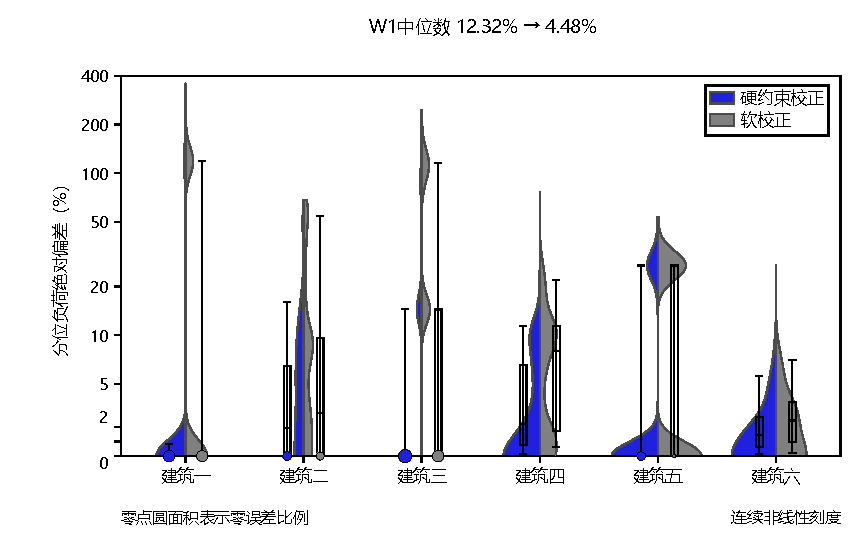
\includegraphics[width=\linewidth]{paper_r2/external_w1.pdf}
\caption{六建筑固定代表日的分布校正。蓝、灰分别表示硬约束与软校正；箱线为加权分位，零点圆面积为零偏差比例。纵轴采用连续非线性刻度，保留完整尾部。}
\label{fig:w1-distribution}
\end{figure}

图\ref{fig:w1-distribution}比较相同累计概率处的原始与代表负荷，展示归一绝对偏差的分布；它反映负荷分布差异，并非逐时预测误差。箱体为25/50/75分位，须为5/95分位，均按原离散概率质量计算。概率加权平均偏差等于对应归一$W_1$；小提琴轮廓仅展示密度。

\begin{table}[htbp]
\centering
\caption{固定代表日集合的权重校正结果}\label{tab:w1}
\begin{tabularx}{\textwidth}{@{}lrrX@{}}
\toprule
建筑 & 软校正误差/\% & 硬约束误差/\% & 硬约束候选的完整准入\\
\midrule
一 & 18.0043 & 4.8097 & 通过\\
二 & 10.0363 & 4.9463 & 原始峰值覆盖不足\\
三 & 20.9090 & 4.1453 & 新增通过\\
四 & 8.2519 & 3.8920 & 通过\\
五 & 14.5937 & 5.4303 & 原始峰值覆盖不足\\
六 & 2.7885 & 2.0065 & 通过\\
\midrule
中位数 & 12.3150 & 4.4775 & 通过数量由3/6增至4/6\\
\bottomrule
\end{tabularx}
\end{table}

六例候选分布误差均下降，中位数由12.3150\%降至4.4775\%，完整统计准入由3/6增至4/6。总能量等式消除加权能量偏差，$W_1$目标调整各负荷水平的出现比例；建筑三因此新增通过。建筑二、五仍因原始峰值覆盖不足被拒绝：调整权重无法补回未保留的峰值。统计准入只检验压缩输入的质量，工程运行可行性仍须通过连续回放校核。

另在已见三城、每城九条固定策略的开发确认中，比较六种权重方法与四档预算。27条连续轨迹共77760小时。硬$W_1$的费用平均绝对百分比误差为0.1405\%，频数法为0.5569\%；实际预算合格选择由9/12增至12/12。其他三种硬方法也达到12/12；这一结果说明压缩质量可以改善固定策略库内的选择，不代表库外全局最优。


\subsection{厂家性能域下的固定设备调度}

TCAV035BHE与TCAV065BHE分别有83、82个Q/P工况点，保留15个缺失角点；同型号有效单元内分别插值制热量Q与输入功率P，再求COP，缺角、越界及跨型号查询均拒绝。在960~m$^2$合成原型上，每城每型号固定一台整机，并固定90~kW电阻补热、80~kW独立制冷和100~kW接入容量。温控基准按当前室温和当小时气象逐时维持舒适范围；LP利用全窗口已给定天气、电价预先安排运行，最小化电量费。六组均覆盖连续2880小时，共用上述资产、20--27~$^\circ$C舒适范围及初末20~$^\circ$C状态。

\begin{table}[htbp]
\centering
\caption{同资产LP相对温控策略的条件运行收益}\label{tab:heatpump}
\begin{tabularx}{\textwidth}{@{}lXrrr@{}}
\toprule
城市 & 型号 & 降费/\% & 节省电量费/元 & 增加电量/kWh\\
\midrule
乌鲁木齐 & TCAV035BHE & 1.3274 & 798.75 & 1398.80\\
乌鲁木齐 & TCAV065BHE & 1.1088 & 474.44 & 753.51\\
固原 & TCAV035BHE & 1.4526 & 908.06 & 1548.64\\
固原 & TCAV065BHE & 1.1013 & 491.80 & 874.83\\
武汉 & TCAV035BHE & 1.1268 & 173.35 & 364.93\\
武汉 & TCAV065BHE & 1.5970 & 237.79 & 728.99\\
\bottomrule
\end{tabularx}
\end{table}

六例电量费降低1.1013\%--1.5970\%，LP目标值与对偶界已按相应编码模型核验。LP在低价时段提前供热，使室温在舒适范围内升高，随后减少高价时段供热；Q/P有效域约束各时段的供热能力与耗电，理想小时占空比表达部分负荷。表\ref{tab:heatpump}所列电量均增加，固定平均因子碳排也随之增加。

\subsection{热容与区域配电约束的交互}

为识别建筑自身的蓄热作用，关闭独立储热，保留两个建筑的温度状态。建筑A固定$H=0.1043$~kW/K、$C=0.535576$~kWh/K；建筑B（图中乙建筑）固定$H=0.15645$~kW/K，仅将$C$从0.535576改为2.142304~kWh/K。另一实验轴为是否施加6.4796375~kW的两楼合计用电上限。四案使用同一武汉气象、2880小时、既有理想设备、20--27~$^\circ$C舒适范围及初末20~$^\circ$C状态；这是热容参数对照，未计现场改造投资。

\begin{table}[htbp]
\centering
\caption{热容倍率与公用电上限的二维对照}\label{tab:factorial}
\begin{tabularx}{\textwidth}{@{}Xrrrr@{}}
\toprule
研究设置 & 电量费/元 & 用电/kWh & 峰值/kW & 绑定小时\\
\midrule
原热容，无公用上限 & 5918.14 & 8155.11 & 14.1064 & ---\\
四倍热容，无公用上限 & 5490.94 & 8725.44 & 25.3335 & ---\\
原热容，有公用上限 & 5937.64 & 8050.61 & 6.4796 & 125\\
四倍热容，有公用上限 & 5660.96 & 8386.07 & 6.4796 & 530\\
\bottomrule
\end{tabularx}
\end{table}

四案均得到求解器容差内最优解，保存的MIP gap为0。共同上限下，增大热容使电量费下降276.68元，即4.6597\%；无共同上限时下降427.20元，即7.2185\%。两项节费之差150.52元，是共同上限削减的热容节费额。共同上限下，区域用电增加335.46~kWh。本组电热设备效率为1，四案无制冷用电且初末温度相同，独立积分核算将该增量分解为建筑A热损减少53.94~kWh、建筑B热损增加389.40~kWh。预热提高室温，也增加向室外散失的热量。

\begin{figure}[htbp]
\centering
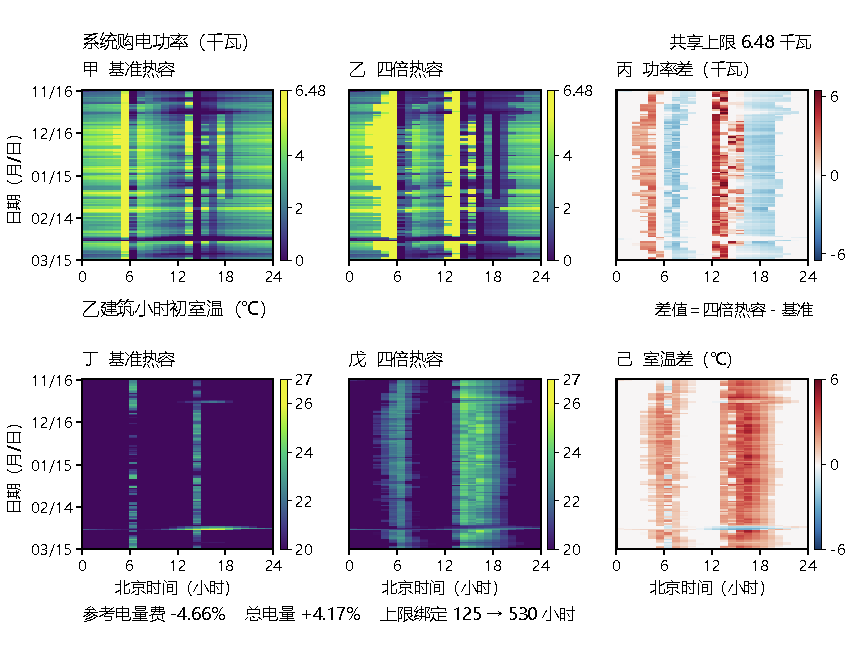
\includegraphics[width=\linewidth]{paper_r2/mechanism_paper/thermal_coupling.pdf}
\caption{共享配电边界下的热惯性调度。上排为系统购电功率，下排为乙建筑小时初室温；第三列为四倍热容减基准。图示完整120日逐时状态，显示预热时移及其容量占用。}
\label{fig:thermal-coupling}
\end{figure}

图\ref{fig:thermal-coupling}将室温变化与购电时移对应起来。绑定小时指两楼合计用电在容差内达到共同上限的小时数，四倍热容使其由125增至530。热容扩大可蓄热空间，也加剧两楼对低价时段容量的竞争，使建筑A的运行与热损随建筑B变化。建筑预热的节费价值因此取决于区域接入容量。

\subsection{管网校核反馈与可行性成本}

在72小时独立泵星型支路参考系统上，固定负荷和设备，在有限稳态模式集合内逐支路检查启用模式的瞬时压降梯度、远端供水温度及逐时热量守恒。将不满足阈值的模式全时段排除后重新优化。表\ref{tab:network}为关闭温差软惩罚的三轮结果，各轮交付热量均为191.5475~kWh。

\begin{table}[htbp]
\centering
\caption{有限网络模式反馈的三轮物理校核结果}\label{tab:network}
\begin{tabularx}{\textwidth}{@{}Xrrr@{}}
\toprule
指标 & 第一轮 & 第二轮 & 第三轮\\
\midrule
最大压降梯度/(Pa/m) & 1081.42 & 504.33 & 237.96\\
最低远端供水温度/$^\circ$C & 61.52 & 59.85 & 57.45\\
管路热损/kWh & 35.70 & 56.94 & 94.44\\
泵耗/kWh & 0.7101 & 0.3570 & 0.1901\\
参考费用/元 & 178.64 & 195.01 & 224.26\\
物理校核 & 压降超限 & 压降超限 & 通过\\
\bottomrule
\end{tabularx}
\end{table}

第三轮满足压降梯度不大于300~Pa/m、远端供水不低于55~$^\circ$C的阈值，得到参考运行费用224.26元的可行方案。排除高流量超限模式后，泵耗与压降下降；较低流量使沿程降温增大、输送同等热量所需启用时间增加，热损与源需求随之上升，费用较第一轮增加25.54\%。反馈给出温压达标的方案及费用代价。第三轮缺少可核验求解下界，所报费用仅作为可行值。

\subsection{三城费用—碳排取舍}

三城另用固定理想资产小原型，以同一温控反馈策略为基准，保持各城天气、舒适和初末状态。费用端点、碳端点分别使电量费、排放最小，中点碳帽取两端排放的平均值。使用共同条件电价与固定平均排放因子；资产与厂家热泵实验不同。表\ref{tab:tradeoff}的降费率以各城基准电量费为分母，增排率以基准排放为分母；节费额保留率为中点节费额除以费用端点节费额。

\begin{table}[htbp]
\centering
\caption{三城中点碳帽方案的决策取舍}\label{tab:tradeoff}
\begin{tabular*}{\textwidth}{@{\extracolsep{\fill}}lrrrr@{}}
\toprule
城市 & 费用端降费/\% & 中点降费/\% & 中点增排/\% & 节费额保留/\%\\
\midrule
乌鲁木齐 & 1.7012 & 1.3916 & 1.7716 & 81.80\\
固原 & 1.7168 & 1.3892 & 1.7469 & 80.92\\
武汉 & 1.7518 & 1.5668 & 2.2003 & 89.44\\
\bottomrule
\end{tabular*}
\end{table}

\begin{figure}[H]
\centering
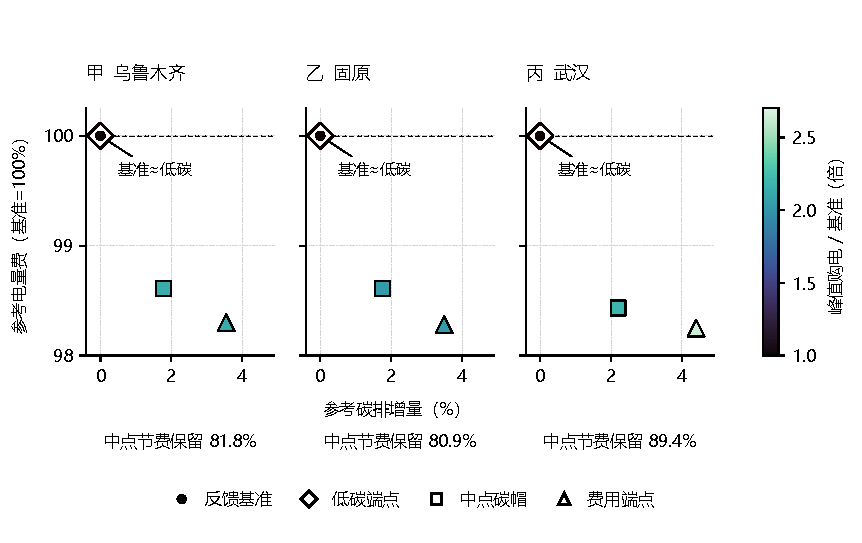
\includegraphics[width=\linewidth]{paper_r2/tradeoff_paper/cost_carbon.pdf}
\caption{三城登记方案的费用、碳排与峰值取舍。图示固定资产实际点，颜色表示峰值与各自基准的比值；中点节费保留率的分母为费用端点相对基准的节省额。}
\label{fig:cost-carbon}
\end{figure}

三城九个优化记录均正常终止，gap不高于$2.63\times10^{-15}$，原运行环境中单记录总耗时3.26--15.27秒。优化点为固定资产问题的容差内最优调度。中点碳帽将费用端点相对基准的增排约减半，同时保留80.92\%--89.44\%的节费额；相对基准仍增排1.75\%--2.20\%。固定平均因子下，碳帽通过限制额外用电，减少可用于低价预热的电量。图\ref{fig:cost-carbon}显示中点峰值仍为基准的2.04--2.21倍，因而排放预算与配电容量需共同考虑。

% !TeX root = ../main.tex
% !TeX program = xelatex
% !TeX encoding = UTF-8
\section{经济评价与方案选择}
\subsection{同口径费用与碳排比较}

表\ref{tab:heatpump}比较相同设备与供热服务下的运行节费，表\ref{tab:tradeoff}比较碳帽下保留的节费额。改变设备配置时，还须判断运行节费能否抵消新增采购和配套费用。

设同等服务下的增量投资为$\Delta I$，年度能源费用节约、新增维护及更新费用分别为$\Delta B_y$、$\Delta M_y$、$\Delta R_y$，期末残值差为$\Delta V_Y$，净现值为
\begin{equation}
\mathrm{NPV}=-\Delta I+\sum_{y=1}^{Y}\frac{\Delta B_y-\Delta M_y-\Delta R_y}{(1+r)^y}+\frac{\Delta V_Y}{(1+r)^Y},
\label{eq:npv}
\end{equation}
其中$r$为折现率，$y$为年度编号，$Y$为评价期年数。该式将未来费用与残值折算到初始时点。下文采用不折现重复窗口比较，求解采购价格阈值。

\subsection{采购价格阈值与方案敏感性}

在相同2880小时服务及固定性能假设下，比较0、1、2台热泵候选，五档碳帽产生三个不同方案。比较费用为采购预算加$F=5$个120日窗口的能源费及假设维护预算，即将同一窗口的运行费用重复计入五次，不折现；$F$不表示五年寿命或回收期。设备价格与性能假设独立于TICA厂家实验。

采购价格对照另不施加碳帽。令$p\geq0$为每台候选设备的采购预算，固定其他条件后，各台数下的最小比较费用可以写成
\begin{equation}
B_0(p)\approx14402.3788,\quad
B_1(p)\approx p+5055.8954,\quad
B_2(p)\approx2p+5455.8596.
\label{eq:price-lines}
\end{equation}
金额均为元，截距来自固定台数下的运行最优解，包含其他采购及重复运行费用。仅改变$p$时，$B_2-B_1\approx p+399.9641>0$，即任一非负价格下两台都比一台更贵。按未截断原值计算一台与零台方案的交点：
\begin{equation}
p^*=B_0(0)-B_1(0)\approx9346.4833\ \text{元}.
\label{eq:price-threshold}
\end{equation}
其余条件固定时，$p<p^*$选择一台，$p>p^*$选择零台，交点处费用相同。阈值表示一台方案除采购价$p$外的费用优势，即最高可支付预算。若一台方案相对零台新增配套投资$\Delta K$、每窗口维护$\Delta M$，其优势条件为\mbox{$p+\Delta K+5\Delta M\leq p^*$}：新增配套和维护费用会占用这份预算。施加碳帽或改变性能、其他费用后需重算费用下包络，即在每个价格处取可行候选费用的最小值。

% !TeX root = ../main.tex
% !TeX program = xelatex
% !TeX encoding = UTF-8
\section{软件组织与可复现性}

程序从天气、建筑、设备和价格配置生成容量、逐时运行、费用与排放结果。\path{src/heatplan/}保存数据检查、模型与求解函数，\path{scripts/}及命令行入口组织实验。配置与核心代码分离，更换城市输入时可复用已有约束；计算前检查对象、单位、时间连续性和允许范围。

核心模块分别处理场景批量计算、代表日权重校正、费用—碳排方案及管网反馈。四段完整伪代码和源文件对应关系见随附\path{supplement/ALGORITHM_DETAILS.md}；其中保留候选失败后的回退检查、限时求解状态及管网排除条件。调用者可据输出状态判断方案是否通过，而非只读取目标值。

2026年10月2日，候选版\texttt{v11.12.0rc6}在独立CPython 3.12.7环境通过252项不重复测试，复算19个连续2880小时案例，包括9个温控、6个固定设备LP和4个容量耦合案例。交付保留依赖锁、运行命令、输入输出字段及校验码。这是既有验收记录；复算时先核对数据和代码版本，再比较逐时结果、费用和约束残差。

% !TeX root = ../main.tex
% !TeX program = xelatex
% !TeX encoding = UTF-8
\section{结论}

本文以统一热量计量、连续建筑状态和物理约束连接供热规划与运行，并用分组实验解释不同决策的作用。

（1）固定代表日后，守恒约束与分布目标仍能改善压缩质量。六楼分布误差中位数由12.32\%降至4.48\%，统计检查通过数由3增至4。三城固定策略库的费用误差由0.5569\%降至0.1405\%，预算合格选择由9/12增至12/12。

（2）完整时序回放与机制对照承担不同任务。四楼历史数学场景完成8784小时服务年和2928小时声明冬季检查；厂家性能域下的三城六组调度降低电量费约1.10\%--1.60\%。双楼中，一楼热容增至四倍时，有、无区域上限的节费金额相差150.52元，表明单楼蓄热价值受共享容量影响。

（3）温压检查能够改变方案。参考管网三轮反馈将最大压降梯度降至237.96~Pa/m，最低远端水温保持57.45~$^\circ$C；相同交付热量下的费用变化可由热损与泵耗解释。

（4）三城中点碳帽保留最低电费方案80.92\%--89.44\%的节费额，并将其额外排放约减半。另在无碳帽、固定性能及$F=5$重复窗口条件下，单台采购预算切换点约9346.48元。两类分析分别为运行取舍和条件采购提供依据。

程序保存输入、配置和逐时结果，方案不仅能比较费用，还能追溯出力、室温及容量占用；替换具体项目参数后可沿用同一检查过程。

\clearpage
\phantomsection
\begin{center}{\heiti\sihao 参考资料}\end{center}
\addcontentsline{toc}{section}{参考资料}
\begin{refsectionflush}
\refentry{1}{中国建筑科学研究院有限公司. 面向供热格局变革的城镇供热源荷匹配与规划寻优模型构建比赛方案{[}R{]}. 2026，第3--5页.}
\refentry{2}{Bacher P, Madsen H. Identifying suitable models for the heat dynamics of buildings{[}J{]}. Energy and Buildings, 2011, 43(7): 1511--1522. DOI: \url{https://doi.org/10.1016/j.enbuild.2011.02.005}.}
\refentry{3}{Madsen H, Bacher P, Bauwens G, et al. Thermal performance characterisation using time series data -- statistical guidelines{[}R{]}. IEA EBC Annex 58, Subtask 3, Part 2. KU Leuven, 2016. \url{https://iea-ebc.org/Data/publications/EBC_Annex_58_Final_Report_ST3b.pdf}.}
\refentry{4}{Kotzur L, Markewitz P, Robinius M, Stolten D. Time series aggregation for energy system design: Modeling seasonal storage{[}EB/OL{]}. arXiv:1710.07593v2, 2018. \url{https://arxiv.org/abs/1710.07593}. DOI: 10.1016/j.apenergy.2018.01.023.}
\refentry{5}{Mavrotas G. Effective implementation of the $\varepsilon$-constraint method in Multi-Objective Mathematical Programming problems{[}J{]}. Applied Mathematics and Computation, 2009, 213(2): 455--465. DOI: 10.1016/j.amc.2009.03.037. 作者配套方法报告：\url{https://www.gams.com/modlib/adddocs/epscm.pdf}.}
\refentry{6}{SciPy developers. scipy.optimize.milp -- SciPy 1.15.3 Reference Manual{[}EB/OL{]}. [2026-10-02]. \url{https://docs.scipy.org/doc/scipy-1.15.3/reference/generated/scipy.optimize.milp.html}.}
\refentry{7}{HiGHS developers. List of options -- HiGHS Documentation{[}EB/OL{]}. 开发版文档，[2026-10-02]. \url{https://ergo-code.github.io/HiGHS/dev/options/definitions/}.}
\refentry{8}{Kersken M, Strachan P. Twin House Experiment IEA EBC Annex 71 Validation of Building Energy Simulation Tools -- Specifications and dataset{[}DS{]}. Fraunhofer Fordatis, version 2, 2020-06-23. CC BY-SA 4.0. \url{https://doi.org/10.24406/fordatis/76.2}.}
\refentry{9}{NASA POWER. Hourly API{[}EB/OL{]}. [2026-10-02]. \url{https://power.larc.nasa.gov/docs/services/api/temporal/hourly/}. 本次响应版本v2.10.2，原始响应、查询及逐字段比对记录随复现资料保存.}

\refentry{10}{Miller C, Kathirgamanathan A, Picchetti B, et al. The Building Data Genome Project 2, energy meter data from the ASHRAE Great Energy Predictor III competition{[}J{]}. Scientific Data, 2020, 7: 368. DOI: \url{https://doi.org/10.1038/s41597-020-00712-x}. 作者版本：\url{https://arxiv.org/abs/2006.02273}.}
\refentry{11}{Judkoff R, Neymark J. International Energy Agency Building Energy Simulation Test (BESTEST) and Diagnostic Method{[}R{]}. NREL/TP-472-6231, 1995. \url{https://www.iea-ebc.org/Data/publications/EBC_Annex_21_BESTEST.pdf}. 本文使用Case 600原型字段及登记的1R1C变换.}
\refentry{12}{TICA. V-FORCE Full DC Inverter Modular Chiller (Heat Pump){[}Z{]}. 24页产品样本，PDF第14--15页（印刷第12--13页）. 经销商存档：\url{https://dec.com.pk/assets/images/products/tica/3-Inverter-modular-chiller.pdf}. 采用冻结副本；出版日期及修订版次未确定.}
\refentry{13}{生态环境部. 2023年电力二氧化碳排放因子{[}Z{]}. 2025，表3. \url{https://www.mee.gov.cn/xxgk2018/xxgk/xxgk01/202512/W020251231726284332528.pdf}. 本文以湖北年平均因子0.4044~kg/kWh作条件比较.}
\refentry{14}{湖北省发展和改革委员会. 关于进一步完善工商业分时电价政策有关事项的通知{[}Z{]}. 鄂发改价管〔2024〕77号. 政府存档：\url{https://www.liangzh.gov.cn/lzhxxgk/xxgkml/ggqsydwxxgk/sdq/202508/P020250825377454860287.pdf}. 月度价格按复现包保存的国家电网湖北2024年11月、12月及2025年1--3月公告取值.}
\end{refsectionflush}

\clearpage
\section*{附录\quad 结果身份与复现入口}
\phantomsection
\addcontentsline{toc}{section}{附录：结果身份与复现入口}
本稿汇总既有研究记录。本次论文复核不新增模型实验。随附\path{EVIDENCE_INDEX.json}给出下列证据编号的完整路径、SHA-256与适用范围；\path{R5_REVIEW.md}逐项对应赛事评分。
\begin{longtable}{@{}p{0.16\textwidth}>{\raggedright\arraybackslash}p{0.79\textwidth}@{}}
\toprule 编号 & 证据与对象\\\midrule
\endfirsthead
\toprule 编号 & 证据与对象（续）\\\midrule
\endhead
\bottomrule\endfoot
E01 & 六楼固定代表日校正；分布误差与统计检查。\\
E02 & 三城两型号厂家设备；六组同资产调度。\\
E03 & 双楼热容与区域容量二维对照；2880小时。\\
E04 & 72小时有限管网模式反馈及各轮物理检查。\\
E05 & 三城费用、碳排及峰值；九条优化记录的状态与耗时。\\
E06 & 无碳帽采购价格阈值；重复窗口条件费用。\\
E07 & 候选版v11.12.0rc6的252项测试与19案例历史复算。\\
E08 & 武汉四楼8784小时服务年及2928小时声明冬季；独立建筑审计和冻结源码。\\
E09 & 三城27条固定策略；六方法、四预算开发确认。\\
\end{longtable}

场景批量、权重校正、多目标与网络反馈的完整伪代码见\path{supplement/ALGORITHM_DETAILS.md}。函数库、配置和逐时输入输出沿用工程目录；新增历史证据摘录的原路径与分发范围均在清单中登记。旧来源审核文件及说明勘误继续保留。
\end{document}
